\begin{abstract}
We study how a feature-learning model acquires \emph{skills} that are presented in context. Targets are additive models
$y=\sum_p c_p\,\sg(\langle v_p,x\rangle)$ with mean-zero task coefficients $c_p$, and a student with learned features and a
linear-in-label attention readout must recover the directions $v_p$ by online SGD from prompts of length $N$. For a single
skill of information exponent $k^*$ we obtain the population loss in closed form. As $N\to\infty$ it is the in-weight loss with the
link squared (effective exponent $2k^*$, a fact implicit in one-step analyses that we make dynamical). At finite $N$ the loss
acquires an \emph{alignment-dependent} variance term $\Gamma^2V(m)/N$, and the way the readout $\Gamma$ is parameterised decides what
this term does: a readout pinned at order one makes the unaligned state drift-stable below $m^*$, so that more prompts cannot
substitute for context length; a free scalar readout shrinks to a Wiener factor, which raises the effective exponent from $2k^*$
towards $4k^*$ and restores a multiplicative trade-off between context length and training time; a readout tied to the feature
norm removes the $N$-dependence altogether. A parameter-free population ODE reproduces the exponents measured by online SGD at
$d=32$ for three readout protocols and four context lengths (11 of 12 cells within $0.6$, the censored cell within $1.0$). With
many skills the dynamics decouple with emergence times $\propto1/\pi_p$; additive compositions of learned skills follow by linearity.
In small softmax transformers we find a $\approx3\times$ per-token handicap of short contexts in the small-alignment regime and the
opposite ordering when the initial alignment is large; these observations are consistent with, but do not test, the mechanism.
\end{abstract}

\section{Introduction}
\label{sec:intro}
Theories of feature learning explain \emph{when} a network acquires a direction $v$ in input space in terms of the information
exponent $k^*$ of the link function~\citep{benarous2021online}: online SGD needs $d^{k^*-1}$ samples ($d\log d$ for $k^*=2$). Theories of
emergence and scaling laws~\citep{michaud2023quantization,nam2024exactly,ren2025emergence} then sum many such acquisitions over
a power-law dictionary of skills. Both lines treat the skill as something learned \emph{in the weights} from a fixed task. Large
models, however, acquire much of their behaviour as \emph{in-context} skills: the pretraining data presents a skill through
prompts whose labels are generated by a task-dependent coefficient, and the network must learn features that make the skill
recoverable from a context of length $N$. Recent analyses of in-context learning with learned features~\citep{oko2024pretrained,
nishikawa2025nonlinear,kim2024transformers,gu2026incontext} treat the context length as an \emph{inference-time} resource: it
controls how well a trained model estimates the task, and in one-step analyses of pretraining it enters only through
concentration, so that more prompts can substitute for longer prompts~\citep[Remark~3]{oko2024pretrained}.

We ask a different question: \emph{does the context length, together with how the readout is parameterised, change which
exponent governs the acquisition of a skill during pretraining?} We answer it in the smallest setting in which the question is
sharp---one or several skills with $k^*=2$ (even links, where in-weight learning is easy), a student with features on the sphere
and a linear-in-label readout, online SGD---and then test the predictions outside the solvable model.

\paragraph{Contributions.}
(1)~\textbf{Closed form.} The population in-context loss of a single feature is
$L_A(m)=1-2\Gamma g(m)^2+\Gamma^2 g(1)\big[(1-\tfrac1N)g(m)^2+V(m)/N\big]$, where $m$ is the overlap with the skill direction,
$g(m)=\E[\sg(\langle v,x\rangle)\sg(\langle w,x\rangle)]$ and $V(m)=\E[\sg^2\sg^2]$ (Prop.~\ref{prop:loss}). As $N\to\infty$ it is the in-weight loss with
$g\mapsto g^2$: the effective exponent is $2k^*$. The $m^{2k^*-1}$ gradient is inside the one-step analysis of
\citet[Lemma~21]{oko2024pretrained} (and depends on parameterisation and initialisation, cf.\ \citet{nishikawa2025nonlinear}); we make
the statement dynamical and verify it by online SGD, including the $k^*=2$ case excluded from \citet{ren2025emergence}.
(2)~\textbf{The finite-context term and the readout} (Props.~\ref{prop:repulsion}--\ref{prop:shrink}). $\Gamma^2V(m)/N$ grows with
alignment. With $\Gamma$ pinned at order one the origin is drift-stable below $m^*$, $m^{*2}=16\Gamma/\big(N(8-4\Gamma(1-\tfrac1N)-24\Gamma/N)\big)$;
under SGD the threshold is soft, and more prompts per step do not remove it (Fig.~\ref{fig:threshold}). With a free scalar
readout, $\Gamma$ moves towards the Wiener value $\Gamma^*(m)=g^2/\big(g(1)[(1-\tfrac1N)g^2+V/N]\big)$ and multiplies the feature gradient:
the effective exponent rises from $2k^*$ towards $4k^*$ as the context statistic becomes noise-dominated; in the adiabatic limit the
escape time scales as $1/N$ there---the multiplicative trade-off of one-step analyses~\citep[Remark~3]{oko2024pretrained} reappears
as a consequence of shrinkage---and at finite readout learning rates the ODE gives an intermediate, parameter-dependent $N$-dependence
that we test prospectively. With the readout tied to the feature norm (the 2-homogeneous student of \citet{ren2025emergence}) the
directional dynamics are norm-independent (their Lemma~B.1) and the $N$-dependence disappears. The population ODE predicts the
exponents measured by SGD at $d=32$ (Fig.~\ref{fig:kappa}).
(3)~\textbf{Many skills and composition.} With a power-law dictionary the dynamics decouple with $T_p\propto1/\pi_p$ (measured slope
$1.44$--$1.53$ for $\pi_p\propto p^{-1.5}$) against $0.75$--$0.89$ for two in-weight baselines, a corollary of (1); additive compositions of
learned skills emerge with the slower skill, by linearity.
(4)~\textbf{Transformers.} In a two-layer softmax transformer with small initial alignment ($d=256$, width 32) a context of 16
with $16\times$ the prompts emerges $\approx3\times$ later than a context of 256 at equal tokens per step; with large initial alignment
($d=32$, width 256) the ordering reverses. Neither pre-registered extreme (a trap; interchangeability) held; we report both as
observations.

\section{Setting}
\label{sec:setup}
Inputs $x\sim\mathcal N(0,I_d)$. A \emph{skill} is a unit vector $v_p\in S^{d-1}$ with link $\sg$; we use the normalised Hermite
polynomials $\sg_k=\mathrm{He}_k/\sqrt{k!}$, so $\E[\sg_j(\langle u,x\rangle)\sg_k(\langle w,x\rangle)]=\delta_{jk}\langle u,w\rangle^k$ for unit
$u,w$ and $k^*=k$. A \emph{task} is a coefficient vector $c$ with independent mean-zero entries, $\E c_p^2=s_p^2$; a \emph{prompt}
consists of $N$ pairs $(x_i,y_i)$ with $y=\sum_p c_p\sg(\langle v_p,x\rangle)$ and a query $(x_q,y_q)$ from the same task. With a
dictionary of $P$ skills and single-skill prompts, skill $p$ appears with frequency $\pi_p$.

\paragraph{Model A (in-context).} Features $\phi_j(x)=\sg(\langle w_j,x\rangle)$, $w_j\in S^{d-1}$, and a linear-in-label readout
\begin{equation}
\hat y_q=\sum_j\Gamma_j\,\phi_j(x_q)\,A_j,\qquad A_j=\frac1N\sum_{i=1}^N y_i\,\phi_j(x_i),
\label{eq:modelA}
\end{equation}
the MLP-plus-linear-attention architecture of \citet{oko2024pretrained}. We consider three readout protocols: \emph{fixed}
$\Gamma_j=\gamma$; \emph{free}, a trainable scalar; and \emph{tied}, $\Gamma_j=\|u_j\|^2$ with $w_j=u_j/\|u_j\|$ (the 2-homogeneous
student of \citet{ren2025emergence}). \textbf{Model B (in-weight)} is ordinary regression $\hat y=\sum_j a_j\phi_j(x)$ on the fixed
task $c\equiv a$. Both are trained by online spherical SGD on the square loss with fresh data at every step: $B$ prompts per step, step size
$\eta$ on the features (renormalised to the sphere after each step), step size $\eta_\Gamma$ on a free readout initialised at $\Gamma_0$,
and for the tied readout an unnormalised $u$ with $\|u_0\|^2=\rho_0$. We report escape times $T_{0.5}$ (steps until $|m|\ge\tfrac12$) and
their \emph{flow-time} version $T_{0.5}\,\eta$, which is what the population ODEs predict; the single-feature experiments initialise
at $m_0=c\,d^{-1/2}$ exactly.

Write $g(m)=\sum_k\alpha_k^2m^k$ for $\sg=\sum_k\alpha_k\sg_k$ and $V(m)=\E[\sg(\langle v,x\rangle)^2\sg(\langle w,x\rangle)^2]=\sum_j\beta_j^2m^j$
where $\sg^2=\sum_j\beta_j\sg_j$. For $\sg_2$: $g=m^2$, $V=1+8m^2+6m^4$.

\section{A single skill}
\label{sec:single}

\begin{proposition}[Population loss]
\label{prop:loss}
For $P=1$, one feature at overlap $m=\langle w,v\rangle$, readout $\Gamma$ and $\E c^2=s^2$,
\begin{equation}
\begin{aligned}
L_A(m)&=s^2\Big[1-2\Gamma g(m)^2+\Gamma^2 g(1)\Big((1-\tfrac1N)g(m)^2+\tfrac{V(m)}{N}\Big)\Big],\\
L_B(m)&=1-2a\,g(m)+a^2g(1).
\end{aligned}
\label{eq:LA}
\end{equation}
\end{proposition}
\begin{proof}[Proof sketch]
Conditional on the task, $A=c\,g(m)+\xi/\sqrt N$ with $\E\xi=0$, $\E\xi^2=c^2(V-g^2)$; $x_q$ is independent of the context, and
$\E[\sg(\langle v,x_q\rangle)\sg(\langle w,x_q\rangle)]=g(m)$, $\E[\sg(\langle w,x_q\rangle)^2]=g(1)$. Expanding $\E(y_q-\hat y_q)^2$ gives~\eqref{eq:LA}.
\end{proof}
We verified~\eqref{eq:LA} by comparing the Monte-Carlo drift $-\E[\partial_wL]\cdot v$ with $-\partial_mL_A$ at $m\in\{0.05,0.1,0.2,0.4\}$ for
$k^*\in\{1,2,3\}$: all 24 points agree within $2.3$ s.e.\ and within $3\%$ for $m\ge0.2$ (Appendix).

\paragraph{The link is squared.} As $N\to\infty$, $L_A=s^2[1-2\Gamma g^2+\Gamma^2g(1)g^2]$ depends on $m$ only through $g(m)^2$, whereas
$L_B$ depends on it through $g(m)$. Near $m=0$ the drift is $2\Gamma s^2(2-\Gamma g(1))\,k^*\alpha_{k^*}^4m^{2k^*-1}$ against
$2ak^*\alpha_{k^*}^2m^{k^*-1}$ for Model B: the label enters the prediction twice---through the context statistic and through the
comparison with $y_q$---and the mean-zero task prior removes the cross terms that would provide a degree-$k^*$ path. (A bias added to $A_j$ would give an in-weight path for the \emph{mean} task only, cf.\ \citet{zhang2024incontext} for the linear case;
we do not analyse it here.)
With the escape heuristics of \citet{benarous2021online} (drift $\eta Cm^{\kappa-1}$, renormalisation drag $-\eta^2dm/2$) the
timescales are $d^{\kappa-1}$ with $\kappa=2k^*$: for $k^*=2$, in-weight needs $d\log d$ samples and in-context $d^3$.

\begin{proposition}[Finite context: a drift-stable unaligned state]
\label{prop:repulsion}
For $\sg_2$ and fixed readout $\Gamma=\gamma$, $-\partial_mL_A=s^2\big[(8\gamma-4\gamma^2(1-\tfrac1N)-24\gamma^2/N)m^3-16\gamma^2m/N\big]$. For
$\gamma<\gamma_1=2N/(N+9)$ the origin is a local minimum of $L_A$, the drift is repulsive for $m<m^*$ and attractive on $(m^*,1)$, with
$m^{*2}=4\gamma/\big(2N-(N+5)\gamma\big)\approx2\gamma/(N(1-\gamma/2))$ (for $\gamma\ge\gamma_1$ the overlap decays from every $m_0<1$);
for general $\sg_k$, $k\ge2$, the same holds with $m^{*\,2(k-1)}\approx2k\gamma/\big((2-\gamma)N\big)$ to leading order, because $\sg_k^2$ has
normalised second Hermite coefficient $\beta_2^2=2k^2$ (Appendix~\ref{app:deriv}).
\end{proposition}
The variance $V(m)$ of the context statistic \emph{grows} with alignment---an aligned feature has heavy tails that coincide
with the teacher's---so the finite-context noise penalises alignment. A feature initialised at $m_0\approx d^{-1/2}$ is attracted
only if $d\lesssim d^*=N(8-4\gamma(1-\tfrac1N)-24\gamma/N)/(16\gamma)$ ($\approx31$ for $\gamma=1$, $N=128$). For $k^*=1$ the repulsion is a constant
fraction $\gamma/N$ of the attraction and is harmless. One-step analyses of pretraining do not see this term because the readout
is initialised at $\gamma\propto d^{-k^*}$~\citep[Lemma~18]{oko2024pretrained}, which makes $\Gamma^2V/N$ negligible; the phenomenon lives where
$\Gamma$ is order one or trained.

\begin{remark}[Soft under SGD]
SGD is a diffusion on the sphere; a run started below $m^*$ escapes with a Kramers-type probability $\sim e^{-\Delta L/D_{\rm eff}}$,
$\Delta L=L(m^*)-L(m_0)$, $D_{\rm eff}=\eta\,\mathrm{Var}(\partial_m\text{-gradient})/2$. At $\gamma=1$, $N=128$: $d=16$ has $m_0>m^*$ (no barrier),
$d=32$ sits on the ridge ($\Delta L/D_{\rm eff}\approx0.02$), $d=64$ is trapped ($\Delta L/D_{\rm eff}\approx20$). Observed escapes in $3\cdot10^5$ steps: $3/3$, $1/3$, $0/3$.
Larger batches lower $D_{\rm eff}$ and \emph{deepen} the trap.
\end{remark}

\begin{proposition}[Readout parameterisation: three regimes---informal summary of Theorems~\ref{thm:A}--\ref{thm:B} and Prop.~\ref{prop:joint}, Appendix~\ref{app:thm}]
\label{prop:shrink}
Consider the population gradient flow of~\eqref{eq:LA} for $\sg=\sg_2$ in flow time $t=\eta\cdot\text{steps}$, started at $m_0=d^{-1/2}$,
and let $\tau_{\rm esc}$ be the time to reach $m=\tfrac12$.
\begin{enumerate}
\item[(a)] \emph{Pinned readout} $\Gamma=\gamma$. The overlap drift is $(8\gamma-4\gamma^2(1-\tfrac1N)-24\gamma^2/N)m^3-16\gamma^2m/N$ (Prop.~\ref{prop:repulsion}).
If $m_0<m^*(\gamma,N)$ then $\tau_{\rm esc}=\infty$; otherwise $\tau_{\rm esc}=\Theta(m_0^{-2})$ with an $N$-dependence that saturates for $N\gg\gamma d$.
The condition involves $N$ and $\gamma$ only---not the number of prompts per step, which does not enter the population drift.
\item[(b)] \emph{Free scalar readout} $\dot\Gamma=-r\,\partial_\Gamma L_A$, $r=\eta_\Gamma/\eta$, $\Gamma(0)=\Gamma_0$. The fixed point of $\Gamma$ at given $m$ is
$\Gamma^*(m)=g^2/\big(g(1)[(1-\tfrac1N)g^2+V/N]\big)$, approached at rate $2r\,g(1)[(1-\tfrac1N)g^2+V/N]\approx2r/N$. \emph{Adiabatic case}
($2r/N\gg$ the overlap rate): the overlap sees $L_A(m,\Gamma^*)$, whose exponent is $4k^*$ for $m^{2k^*}\ll V/N$ and $2k^*$ otherwise, and in the
former regime $\tau_{\rm esc}\propto m_0^{-(4k^*-2)}/N$ (Appendix~\ref{app:deriv}). \emph{Growth-limited case} ($2r/N\lesssim$ the overlap rate; E2 at $N=16$ is adiabatic to $1\%$, the other cells are not): $\Gamma$ lags $\Gamma^*$ and $\tau_{\rm esc}$ depends on $(N,\Gamma_0,r)$ jointly; the ODE gives intermediate
$N$-dependences (e.g.\ $\tau(16)/\tau(256)=4.4$ at $d=64$, $\Gamma_0=0.01$, $r=1$, against $16$ in the adiabatic $1/N$ law).
\item[(c)] \emph{Tied readout} $\Gamma=\rho=\|u\|^2$, features $\sg(\langle u/\|u\|,x\rangle)$. The directional velocity is
$(1-m^2)\big[4gg'-\rho\,(2(1-\tfrac1N)gg'+V'/N)\big]$, which is exactly the pinned velocity at $\gamma=\rho$ divided by $\rho$ (norm-independence
of the attraction, \citealp[Lemma~B.1]{ren2025emergence}): a tied readout behaves like a pinned readout of value $\rho(t)$ under a time
change. From a small $\rho_0$, $\dot\rho=-4\rho\,\partial_\rho L_A$ leaves $\rho$ near $\rho_0$ and $\tau_{\rm esc}=\Theta(m_0^{-2})$ is independent of
$N$---the tied readout self-selects the small-readout regime. Let $\rho^*(m)=2Nm^2/\big(4+(N+5)m^2\big)\approx Nm^2/2$ be the value at which the
directional drift vanishes. For $\rho_0>c_2\rho^*(m_0)$, $c_2=\tfrac43$ (Theorem~\ref{thm:A}(iii); between $\rho^*$ and $c_2\rho^*$ the overlap first
falls and then escapes), the population flow traps permanently ($m\propto t^{-2}$ while $\rho\propto t^{-1}$, so $\rho$ never falls below the
moving threshold); under SGD,
noise keeps $m$ at the noise floor while $\rho$ decays, and the feature is eventually released---a long delay rather than a trap (E5).
\end{enumerate}
\end{proposition}
Integrating the population flow confirms the three regimes quantitatively (Appendix~\ref{app:deriv}): for $\sg_2$ at $d=512$ and
$N=32,128,512$ the escape times are $\infty,771,386$ (pinned $\gamma=0.1$), $9.0\cdot10^4,2.2\cdot10^4,5.4\cdot10^3$ with $\tau N=2.9,2.8,2.75\times10^6$
(free), and $39,34,33$ (tied); at $d=32$ the statistic is signal-dominated for $N\gtrsim d^{k^*}=1024$ and $\tau=52,37,34,33$ for $N=32$--$2048$.
The static value $\Gamma^*$ is the ridge/Wiener optimum that appears in replica analyses of trained
models~\citep[eqs.~(297)--(298)]{gu2026incontext}; our point is its \emph{dynamical} effect: the same loss yields a trap, a multiplicative $N$--$T$ trade-off (that of
\citet[Remark~3]{oko2024pretrained}) with an exponent crossover, or no $N$-dependence, according to the readout. That a fast readout doubles the exponent of an in-weight problem is
known~\citep[\S5]{bietti2023learning}; what is specific to the in-context problem is that the finite-context noise drives the
readout towards $\Gamma^*$, so that \emph{whether context length trades off against training time, is irrelevant, or is a
hard requirement is decided by how the readout is parameterised}. One-step analyses have a readout initialised at $\gamma\propto d^{-k^*}$~\citep[Lemma~18]{oko2024pretrained}, which makes $\Gamma^2V/N$
negligible and places them in the regime where only the product of prompts and prompt length matters.

\paragraph{E1: exponents by SGD.}
Online SGD, $\sg_2$, $d=32$, $\eta=1/d^2$, initial overlap $m_0=c\,d^{-1/2}$, $c\in\{0.5,0.7,1,1.4\}$, three seeds each; the escape
time from $m_0$ scales as $m_0^{-(\kappa-2)}$ for $\kappa>2$, so the slope of $\log T_{0.5}$ against $\log m_0$ estimates $\kappa_{\rm eff}=2-\text{slope}$
(12 runs per cell; the estimator is coarse and the censored cells are biased low). Fig.~\ref{fig:kappa} shows $\kappa_{\rm eff}$ for free
($\eta_\Gamma=\eta$ and $10\eta$) and tied readouts at $N\in\{32,128,512,4096\}$ against the population ODE of
Props.~\ref{prop:loss}--\ref{prop:shrink} (integrated with LSODA, rtol $10^{-10}$; an earlier Euler integrator overestimated times by
$0.6$--$3.6\%$ without changing any exponent or trap verdict) evaluated \emph{after the run} at the same $d$, $m_0$-grid, $\Gamma_0$ and $\eta_\Gamma/\eta$ (the ODE
itself was fixed before the run; its evaluation at these parameters was not pre-registered): tied $4.10$--$4.44$ (ODE $4.15$--$4.18$); free
$4.8$--$6.6$ rising as $N$ falls (ODE $4.85$--$7.0$). With a censored (Tobit) fit for the three cells that contain censored runs, all twelve cells agree with the ODE within $0.5$
(ordinary least squares on reached runs only: eleven within $0.6$, the free $N=32$, $\eta_\Gamma=\eta$ cell $1.0$ low); the estimator is a
secant over a factor $2.8$ in $m_0$ and local slopes vary, so these are effective, not asymptotic, exponents, and the prompts per step
were $32$ for $N\le128$ and $8$ for $N\ge512$ (a $B=8$ control at $N=128$ gives $5.38\pm0.26$ vs $5.59\pm0.20$). The ODE also
reproduces absolute escape times: over the 45 fully-reached E1 cells the ratio median-SGD/ODE lies in $[0.64,1.34]$ with 24 within
$10\%$ and 35 within $20\%$ (no trend in $N$ or protocol; the largest deviations are at the smallest $m_0$), and one censored cell
(free, $10\eta$, $N=128$, smallest $m_0$) is at least $2.3\times$ slower than predicted (Appendix~\ref{app:exp}). The
in-weight model at the same $k^*$ gives a logarithmic $m_0$-dependence ($\kappa=2$). $\kappa_{\rm eff}$ is a secant over a factor $2.8$ in $m_0$ at fixed $(d,N,\Gamma_0,\eta_\Gamma/\eta)$, not an asymptotic exponent: at fixed $N$ and
$d\to\infty$ the free-readout flow gives $4k^*$ for every $N$ with $N$ only in the prefactor (Theorem~\ref{thm:B}:
$\tau_{\rm esc}\sim e^{(4k^*-2)k^{*2}\Gamma_0^2/r}\,\mu_0^{-(4k^*-2)}d^{2k^*-1}/(4k^*(4k^*-2)N)$), while a $d$-free limit exists under the joint
scaling $\lambda=N/d^{k^*}$, $\tilde r=(\eta_\Gamma/\eta)/d$, giving $\kappa(\lambda,\tilde r,\Gamma_0)$ whose $d\to\infty$ values ($6.45/5.40/4.95/4.83$)
are within $0.06$ of the $d=32$ ODE numbers; its large-$\lambda$ end at small $\Gamma_0$ is $2k^*+1$ (readout growth from $\Gamma_0$), not $2k^*$.
The pre-registered ``$4\to8$'' was this corner structure misstated as $d\to\infty$ limits. Two pre-registered predictions in this experiment failed and are
reported as such: the learned $\Gamma$ at $T_{0.5}$ is $0.18$--$0.25$, below $\Gamma^*(0.5;N)=0.38$--$0.99$ (the readout has not equilibrated at
$\eta_\Gamma=\eta$; the exponent prediction does not depend on this), and a scan of $T_{0.5}$ against $d\le48$ at $N=128$ versus $2048$ showed
no $N$-dependence (slopes $3.49\pm0.08$ vs $3.70\pm0.21$), which is what the ODE predicts for $d\le48$ but means the $N$-dependence is
established only through $\kappa_{\rm eff}(N)$ at fixed $d$. With the tied readout at $\rho_0=1$, $N=128$, the natural O(1)-readout
version of Prop.~\ref{prop:repulsion}, $d=32$ escaped ($3/3$) while $d=64$ was trapped ($0/3$, $\rho$ decaying to $0.18$).

\paragraph{E2: the three regimes by SGD (the prospective test of Prop.~\ref{prop:shrink}).}
To test Prop.~\ref{prop:shrink} directly (Fig.~\ref{fig:regimes}) we fix $d=64$, $m_0=d^{-1/2}$, $\eta=1/d^2$, vary $N\in\{16,64,256\}$ under two schemes---tokens per
step fixed ($NB=4096$) and prompts per step fixed ($B=64$)---and run the four protocols, three seeds each, with the population
escape times computed before the run. Pinned $\gamma=1$: no escape at $N\le64$ in $10^6$ steps ($0/9$, including $B=256$), $3/6$ at $N=256$
($d^*\approx63$); pinned $\gamma=0.1$: median $396$k$/192$k$/179$k steps against $400$k$/193$k$/175$k predicted; free: $1.78$M$/614$k$/402$k
against $1.84$M$/627$k$/414$k, ratio $T(16)/T(256)=4.4$ ($3.6$--$5.0$ over seed pairings) as predicted ($4.44$)---the growth-limited value of
Prop.~\ref{prop:shrink}(b), not the adiabatic $1/N$ law; tied: $17.0$k$/15.1$k$/14.0$k against $17.0$k$/16.4$k$/16.3$k (flat within $\times1.25$,
seed pairings $0.9$--$1.45$). Three seeds resolve medians to roughly $5\%$. In every protocol the two batch schemes give the same step counts,
as they must at fixed step size (the population drift does not contain $B$); the trade-off is between context length and the number of
SGD steps, and a step size scaled with $B$ is tested in Appendix~\ref{app:exp}. (The free-readout $N=16$ cells exceeded the pre-registered
$10^6$-step cap, as the ODE had predicted, and were rerun to $2.5\cdot10^6$ steps.)



\paragraph{E5: controls.}
Varying the readout's initial value and learning rate (free: $\Gamma_0=0.1$ or $\eta_\Gamma=10\eta$ at $d=64$) changes the $N$-ratio from $4.4$ to
$9.2$ and $10.7$ (ODE $9.1$ and $8.9$; medians within $2\%$ except the $\eta_\Gamma=10\eta$, $N=16$ cell, $24\%$ slow), confirming that the
free-readout exponent is a function of $(N,\Gamma_0,\eta_\Gamma/\eta)$, as Prop.~\ref{prop:shrink}(b) states. A pinned $\gamma=0.01$ readout is as
$N$-flat as the tied one (ratio $1.06$, ODE $1.04$). A tied readout started at $\rho_0=0.3>\rho_{\rm trap}(m_0)=0.18$ at $N=16$ was pre-registered to trap
(the deterministic flow provably does, Theorem~\ref{thm:A}(iii): $m\propto t^{-2}$, $\rho\propto t^{-1}$); under SGD all three seeds escaped after a $\approx30\times$ delay, once $\rho$ had
decayed to $0.012$---so under SGD tying converts the pinned trap into a delay, and the pre-registered wording "the repulsion survives tying" is
withdrawn in favour of "is delayed by tying". Finally, scaling the step size with the batch ($\eta\propto B$, pinned $\gamma=0.1$, $N=64$)
leaves the escape \emph{flow time} invariant to $0.5\%$ while steps scale as $1/\eta$: the irrelevance of prompts per step in E2 is a
statement about flow time, independent of how $\eta$ is chosen.

\begin{figure}[t]
\centering
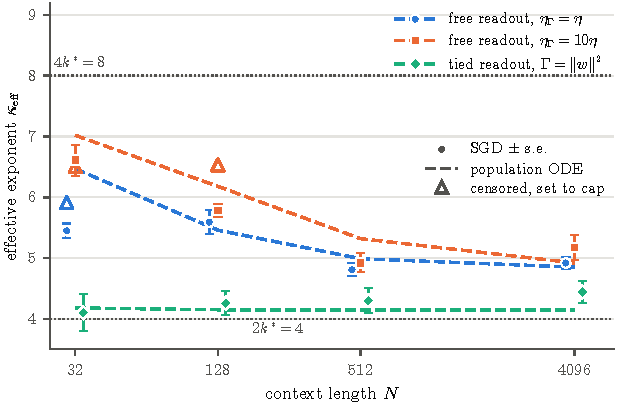
\includegraphics[width=.63\linewidth]{figs/fig_kappa.pdf}
\caption{Effective exponent of skill acquisition for $k^*=2$ at $d=32$: online SGD (points, $\pm$s.e.; triangles: censored runs
set to the step cap) against the parameter-free population ODE (dashed). The tied readout stays at $2k^*=4$; the free readout
rises towards $4k^*=8$ as the context shortens.}
\label{fig:kappa}
\end{figure}

\begin{figure}[t]
\centering
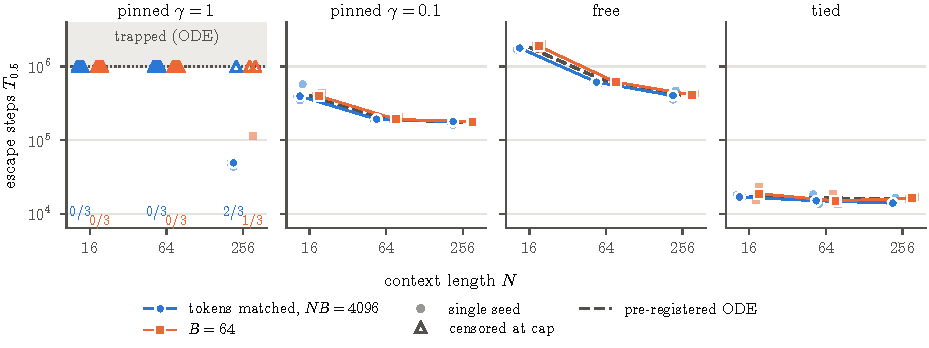
\includegraphics[width=.985\linewidth]{figs/fig_regimes.pdf}
\caption{Escape steps $T_{0.5}$ (first step with $|m|\ge0.5$) against context length $N$ for the four readout protocols ($d=64$, $\eta=1/d^2$,
$m_0=d^{-1/2}$; shared log--log axes). Light markers are single seeds (three per cell), solid markers and lines the median over seeds, for
tokens per step fixed ($NB=4096$, circles) and prompts per step fixed ($B=64$, squares). Open triangles are runs that had not escaped at the
step cap ($10^6$) and are drawn at the cap; the counts under the pinned-$\gamma=1$ panel are runs escaped out of $3$. Dashed lines are the
population-ODE escape times (flow time $\times d^2$), \emph{fixed before the run}; pinned $\gamma=1$ has no finite ODE escape time
(trapped, shaded beyond the cap). The free-readout $N=16$ cells use the reruns to $2.5\cdot10^6$ steps (the pre-registered cap was
exceeded by the predicted $1.84$M steps). At $N=64$ both schemes have $B=64$ and are the same three runs.}
\label{fig:regimes}
\end{figure}

\begin{figure}[t]
\centering
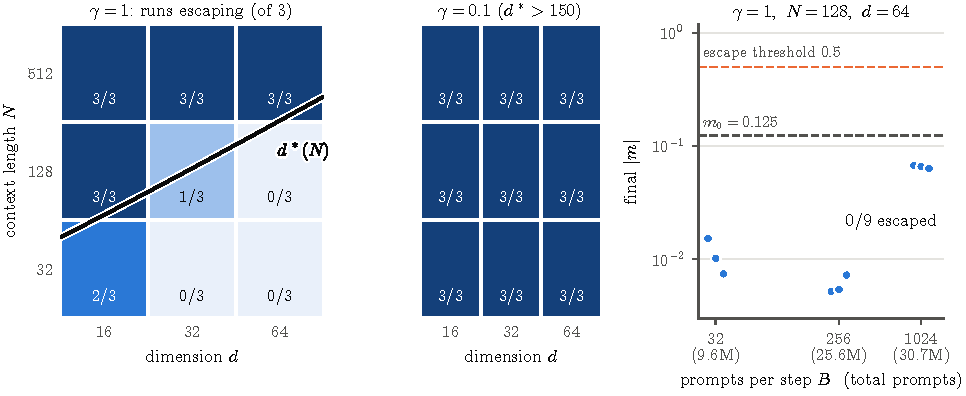
\includegraphics[width=\linewidth]{figs/fig_threshold.pdf}
\caption{Left: fraction of runs escaping $m_0=d^{-1/2}$ within $3\cdot10^5$ steps (fixed readout, 3 seeds per cell; curve: $d^*(N)$ of
Prop.~\ref{prop:repulsion}; for $\gamma=0.1$ the curve lies above the grid). Right: at $\gamma=1$, $N=128$, $d=64$ no run escapes for
$B\in\{32,256,1024\}$ prompts per step (total prompts $\times1$, $\times2.7$, $\times3.2$) and the final overlap falls \emph{below} $m_0$:
more prompts do not substitute for context length.}
\label{fig:threshold}
\end{figure}

\section{Many skills and composition}
\label{sec:many}
Fig.~\ref{fig:many} summarises Exps.~2--3. With $P$ orthogonal skills and $M\ge P$ features the loss splits, when each feature is assigned to one skill, into
$\sum_p\pi_p s_p^2\,\ell(m_p)$ with $\ell$ the single-skill loss; each overlap then follows the single-feature dynamics with rate
$\propto\pi_ps_p^2\Gamma$, so $T_p\propto1/\pi_p$. In-weight learning of the same dictionary carries the coefficient $a_p$ (with
$a_p^2\propto\pi_p$), hence $T_p\propto1/a_p\propto\pi_p^{-1/2}$: in-context learning orders skills by frequency about twice as steeply---a corollary of the squared link,
since the in-context drift carries $\E c_p^2\,\pi_p$ and the in-weight drift carries $a_p$.
\textbf{E3} ($d=32$, $P=16$, $\pi_p\propto p^{-1.5}$, $M=64$, fixed $\Gamma=0.1$, three seeds) gives slopes of $\log T_p$ versus $\log p$ of
$1.44\pm0.08$ (drop midpoints; $1.53\pm0.22$ with the $0.5$-crossing) for the in-context model, against $0.75\pm0.08$ for a capacity-matched in-weight baseline and $0.75$--$0.89$ for the
2-homogeneous in-weight student of \citet{ren2025emergence} (small initialisation, no hand-chosen readout; the lower value is
limited by the logging resolution, the higher one uses a dense early log). Both in-weight baselines fit the target
\emph{collectively} at $M=64>d$ (every skill shared by $\ge2$ features, pooled alignment $\to1$, no single feature above $0.9$), so the
in-weight slope is an empirical baseline rather than a decoupled-neuron prediction; its emergence times nonetheless obey
$T_p\,\eta\,a_p=\mathrm{const}$ ($0.23$--$0.26$ across skills and three learning rates), i.e.\ ordering by the coefficient $a_p\propto\sqrt{\pi_p}$,
whereas the in-context times obey $T_p\,\eta\,\pi_p m_0^2=\mathrm{const}$. The
constant $T_{p}\,\eta\,\pi_p m_0^2=0.73$ (IQR $0.70$--$0.77$) across skills and seeds equals the single-feature value ($0.64$), i.e.\ the
many-skill dynamics is the single-feature dynamics with rate $\pi_p$. Per-skill drops are $\approx4\times$ sharper than in-weight
(relative width $1.08$ vs $4.09$). The frequency-weighted alignment loss decays as $t^{-0.40\pm0.04}$ over the window in which skills
3--8 emerge, against $(\alpha-1)/\alpha=0.33$ for an idealised staircase; the window spans only a factor 3--8 in time, so the exponent
depends on the emergence definition and we do not claim a scaling-law ratio.

\paragraph{E4: composition.} Because~\eqref{eq:modelA} is linear in the context labels, $\hat y_q(c_1,c_2)=\hat y_q(c_1,0)+\hat y_q(0,c_2)$
identically, and for independent mean-zero $c_1,c_2$ the loss on an additive pair is the sum of the single-skill losses. Trained on
single-skill prompts only ($d=32$, $P=2$, $\pi=0.75/0.25$, $M=4$), the pair
loss reaches $90\%$ of its drop before or together with the slower skill in every run (never after)---which is forced by
linearity, so this is a check of the identity under SGD, not a test; on a thresholded accuracy, where \citet{arora2023theory}
predict an extra delay for tuples, the
thresholded pair accuracy is approximately the product of the single-skill accuracies ($\mathrm{acc}_{12}\approx0.85\,\mathrm{acc}_1\mathrm{acc}_2+0.09$, r.m.s.\
$0.008$ from $y=x$)---the multiplicative form observed empirically by \citet{okawa2023compositional}, and a delay of the kind
\citet{arora2023theory} describe---while a Gaussian-error closed form fails (heavy tails). A product composition
$\sg_1(\langle v_1,x\rangle)\sg_1(\langle v_2,x\rangle)$ is not learned (loss $\approx1$), as expected for a model never shown product prompts.

\begin{figure}[t]
\centering
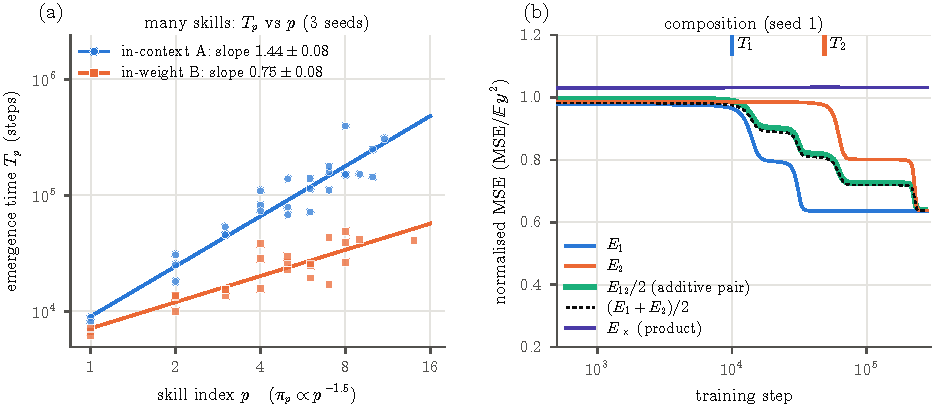
\includegraphics[width=\linewidth]{figs/fig_many.pdf}
\caption{(a) Emergence time (drop midpoint) of skill $p$ versus skill index for the in-context model (slope $1.44\pm0.08$), the
capacity-matched in-weight baseline (slope $0.75\pm0.08$) and the 2-homogeneous in-weight student (slope $0.75$--$0.89$), $\pi_p\propto p^{-1.5}$,
three seeds each; unlearned skills omitted.
(b) Composition (Exp.~3, one seed): normalised MSE on skill-1 prompts, skill-2 prompts, the additive pair (halved) and the product
pair; the dotted curve is half the sum of the single-skill losses and lies on the pair curve. Plateaus at $0.64$ are the fixed-readout
floor $(1-\Gamma n)^2$, not zero.}
\label{fig:many}
\end{figure}

\begin{figure}[t]
\centering
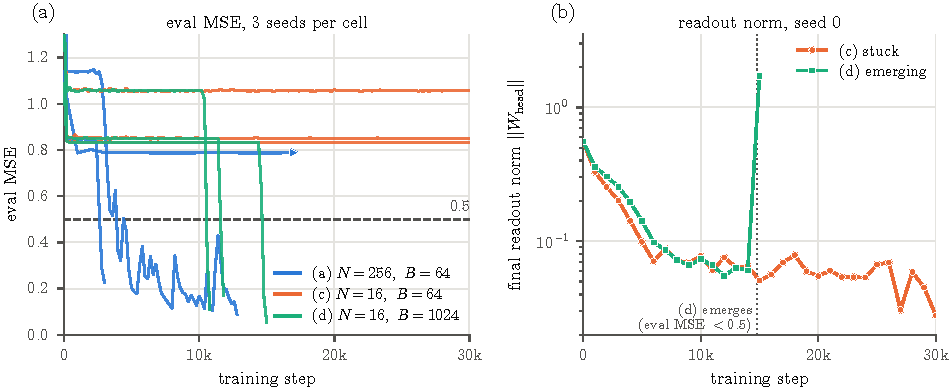
\includegraphics[width=\linewidth]{figs/fig_transformer.pdf}
\caption{Two-layer softmax transformer, $d=256$, MLP width 32, $k^*=2$. (a) Evaluation MSE for $N{=}256,B{=}64$; $N{=}16,B{=}64$; and
$N{=}16,B{=}1024$ (same tokens per step as the first), three seeds each; one $N{=}256$ seed was censored at $17$k steps on the plateau.
(b) Norm of the final readout for one stuck run ($N{=}16,B{=}64$) and one emerging run ($N{=}16,B{=}1024$, same seed): the norm
collapses while the skill is unlearned; the regrowth at emergence is a single logged point (norms logged every $1000$ steps).}
\label{fig:transformer}
\end{figure}

\section{Transformers: where the effect shows and where it does not}
\label{sec:transformer}
We train two-layer softmax transformers (4 heads, pre-LN, Adam, online data; Fig.~\ref{fig:transformer}) on the same in-context task with $k^*=2$ and ask
whether a short context can be compensated by more prompts per step. \textbf{Large initial alignment} ($d=32$, MLP width 256; the best
of 256 random first-layer directions already has $|\cos|=0.43$--$0.55$ with $v$): at a fixed $8192$ tokens per step the emergence step
\emph{increases} with $N$ ($1000/1400/2800$ for $N=16/64/256$)---fewer prompts per step dominate and the mechanism is invisible, as it
must be when $m_0\gg m^*$. \textbf{Small initial alignment} ($d=256$, width 32; $|\cos|_0=0.13$--$0.18$): $N=16$ with $B=64$ prompts never
emerges in $30$k steps ($3/3$); $N=16$ with $B=1024$ (the same tokens per step as $N=256$, $B=64$) emerges in all seeds but at
$10.6$--$14.8$k steps, $\approx3\times$ later than $N=256$ ($2.8$--$4.0$k); while a run is on the plateau its final readout norm collapses from $0.57$ to
$0.03$--$0.16$ (in stuck and emerging runs alike), and the first norm logged after emergence is back at $1.7$. Neither pre-registered extreme (a trap, or interchangeability of $N$ and $B$) holds; the $\approx3\times$ ratio rests on two paired seeds,
the Adam step was not rescaled with $B$, and the readout collapse is identical in stuck and later-emerging runs (Fig.~\ref{fig:transformer}b),
so it is plateau behaviour rather than a signature of Prop.~\ref{prop:shrink}. We state the result as an observation consistent
with---not a test of---the mechanism of Sec.~\ref{sec:single}; $k^*=1$ and in-weight controls emerge within $1.4$k and $0.4$k steps.

\section{Related work}
\label{sec:related}
\citet{oko2024pretrained} analyse the architecture~\eqref{eq:modelA} with one gradient step; the product of two correlations
($\propto m^{2Q-1}$) is in their Lemma~21 and the exponent $2Q$ in their total sample count $N_1T_1=\tilde\Omega(d^{2Q+1}r)$, framed as a
consequence of correlational information; their Remark~3 states the $N_1$--$T_1$ trade-off, which Prop.~\ref{prop:shrink} recovers for a shrinking readout and which fails for
a readout pinned at order one (Prop.~\ref{prop:repulsion}, Fig.~\ref{fig:threshold}). \citet{nishikawa2025nonlinear} show that softmax's label
nonlinearity lowers the \emph{inference-time} context length to the generative exponent while one-step pretraining stays at
$d^{\Theta(\mathrm{ie})}$. \citet{gu2026incontext} derive, by the replica method for trained models with $k^*=1$, the kernel-vs-feature
context-length scalings (their feature learner has a single transition at $N=\Theta(d)$, the same scaling as our $d^*(N)$ but for
inference, not for feature emergence) and the static shrinkage $\Gamma^*$ (their eqs.~(297)--(298)); they list jointly trained readouts
and $k^*\ge2$ as open, which is where our results sit. \citet{kim2024transformers} note that at finite sample size the ICL landscape may acquire a spurious minimum at the
origin (their App.~C.4), a qualitative precursor of Prop.~\ref{prop:repulsion}. \citet{ren2025emergence} treat the additive model
in-weight for even links with $k^*>2$ with a 2-homogeneous student; our tied protocol is theirs, the norm-independence of the
directional dynamics is their Lemma~B.1, and $k^*=2$ is outside their assumptions (the companion work \citet{benarous2025quadratic} treats the quadratic case in-weight with a student
narrower than $d$, sample complexity $d\,\mathrm{polylog}\,d$, and notes that the $k\ge3$ decoupling argument does not apply at $k=2$). The doubling of the exponent by a fast link is in \citet[\S5]{bietti2023learning} and \citet{bietti2022learning}; two-timescale
readout dynamics in two-layer networks are analysed by \citet{berthier2023learning}, and \citet[Cor.~2.3]{ren2025emergence} give an
in-weight scaling law in which the frequency ordering is also steepened by the learning-rate schedule.
\citet{zhang2024incontext} prove, for linear regression, that the task mean is learned in-weight by the MLP and the covariance
in-context. Skill-based accounts of emergence~\citep{michaud2023quantization,nam2024exactly,arora2023theory,okawa2023compositional}
are in-weight; our composition result is the label-linear in-context counterpart. Compositions that are not output-additive need extra structure~\citep{kobayashi2024compositional,wang2026power}; \citet{he2024learning}
show that even a label-linear in-context algorithm is not free when the network must discover it against an in-weight memoriser,
whereas in~\eqref{eq:modelA} linearity in the labels is built in.

\section{Limitations}
\label{sec:limits}
The theory is for one feature per skill and $k^*=2$; the SGD threshold is soft; the many-skill statements rest on decoupling,
which fails for rare skills when no feature starts closest to them (2/10 seeds in Exp.~3); the Gaussian closed form for
compositional accuracy is wrong; the transformer results are observational and were pre-registered with predictions that failed in
both directions. All predictions, outcomes and deviations (including two algebra slips corrected after pre-registration and two
ill-posed estimators) are listed verbatim in the appendix.

\paragraph{Reproducibility and disclosure.} Code, pre-registration document and all runs: \todo{repo}. AI assistance was used for
literature search, implementation, derivation checking and drafting; every derivation was verified against the Monte-Carlo drift,
and every citation against the full text.

